\documentclass[a4paper,11pt]{article}
\usepackage[utf8]{inputenc}
\usepackage[russian]{babel}
\usepackage[T1]{fontenc}
\usepackage{amssymb,amsmath,graphicx,indentfirst}
\usepackage{caption}
\usepackage{color}
\usepackage{listings}
\usepackage[unicode]{hyperref}
\usepackage{qtree}

\setlength{\parskip}{1ex plus 0.5ex minus 0.2ex}
\captionsetup[figure]{labelformat=empty}
\captionsetup[figure]{justification=centering}
\lstset{keywordstyle=\color{blue}\bfseries}
\lstset{extendedchars=false, language=Caml, defaultdialect=[Objective]Caml}
\newcommand\doubleplus{+\kern-1.3ex+\kern0.8ex}

\author{Олег Смирнов\\
\texttt{oleg.smirnov@gmail.com}}
\date{18 ноября 2011 г.}
\title{Введение в функциональное программирование -- Лекция 9. Списочные
гомоморфизмы. Третья теорема о гомоморфизмах. Технология MapReduce}

\begin{document}
\maketitle
\tableofcontents
\newpage

\section*{Цель лекции}
\begin{itemize}
\item Списочные гомоморфизмы
\item Третья теорема о гомоморфизмах
\item MapReduce как система для параллелизации вычислений
\end{itemize}

\section{Задача о графе связей}
Пусть задана корпоративная структура некоторой компании в виде графа связей.
Дуга от вершины $A$ к вершине $B$ означает, что сотрудник $A$ подчиняется 
сотруднику $B$. Необходимо найти, кто в компании самый главный, т.е. директора.

Для графа без циклов, т.е. для дерева, задачу можно решить топологической
сортировкой за $O(|V| + |E|)$ итераций, где $|V|$ -- количество вершин, а
$|E|$ -- количество связей. Топологическую сортировку можно получить, например,
из поиска в глубину.

\begin{figure}[h]
    \begin{center}
        \includegraphics[height=130mm]{lecture9/orgchart.eps}
        \caption{Корпоративные структуры}
    \end{center}
\end{figure}

А как быть, если в графе присутствуют циклы? В общем виде, пусть есть граф,
где вершины -- это люди, а дуги -- некоторые связи между ними. Например,
в социальной сети дуга может описывать отношение $A$ (Алиса) ``добавила в 
друзья'' $B$ (Боба). Задача: выявить наиболее ``влиятельных'' людей в такой
сети. Эта задача имеет массу применений на практике. Например, в рекламе и
маркетинге.

Очевидно, что ``влиятельность'' можно определять разными способами. Можно просто
подсчитывать количество друзей. Предположим, что Алису добавило в друзья
десять человек, а Боба -- всего три. Но у каждого из троих друзей Боба есть
ещё по сотне своих друзей. В этом случае наша формула посчитает Алису более
``влиятельной'', хотя на деле ситуация противоположная.

Идея: определим меру влиятельности рекурсивно. Т.е. для некоторого пользователя
$p$ определим влиятельность $I(p)$ пропорционально влиятельности его друзей, т.е.
\begin{equation*}
  I(p) = \alpha (I(f_1) + I(f_2) + \ldots + I(f_k))
\end{equation*}
где $f_1 \cdot f_k$ -- друзья $p$, а $\alpha > 0$ -- некая константа.

Представив социальный граф в виде матрицы смежности 
$A \in \mathbb{R}^{n \times n}$, можно записать формулу:
\begin{equation*}
  I(p_i) = \alpha \sum_{j} A_{ij} I(p_j)
\end{equation*}
Легко видеть, что функция $I$ принимает $n$ возможных значений, т.е. является
вектором $\vec{x} \in \mathbb{R}^n$. Пусть $\lambda = \frac{1}{\alpha}$. Тогда
\begin{equation*}
  \vec{x} = \alpha A \vec{x}
\end{equation*}
\begin{equation*}
  A \vec{x} = \lambda \vec{x}
\end{equation*}
Проще говоря, задача свелась к поиску собственного вектора $\vec{x}$ для матрицы
смежности $A$ для некоторого собственного числа $\lambda > 0$. Можно показать,
что искомый вектор соответствует наибольшему из собственных чисел матрицы.

Эта задача называется ``eigenvector centrality''. В общем случае, ``centrality''
-- это некий (возможно, частичный) порядок на множестве вершин графа, т.е.
функция 
\begin{equation*}
  \mu: V \rightarrow \mathbb{R}
\end{equation*}
Сумма всех связей вершины называется ``degree centrality''. В нагруженном
графе можно взять значение, обратно пропорциональное сумме весов связей --
получится ``closeness centrality'' и т.д.

Разновидностью ``eigenvector centrality'' является алгоритм PageRank,
который лежит в основе поискового движка компании 
Google~\cite{Page99thepagerank}. В его модели используется некоторый 
гипотетический пользователь, который нажимает на ссылки в браузере в 
случайном порядке. ``Важность'' страницы определяется как вероятность попадания
на неё этим ``случайным'' пользователем.
\begin{enumerate}
\item Интернет можно представить в виде матрицы смежности, где вершинами
  будут страницы, а рёбрами -- ссылки между ними.
\item Такую матрицу смежности можно нормализовать, разделив значения в
  каждой строка на сумму значений этой строки, если она не равна нулю.
  Полученная матрица описывает марковский процесс для нашей модели
  со ``случайным'' пользователем.
\item Искомый вектор вероятностей -- это ``предел'' марковского процесса
  или состояние равновесия.
\end{enumerate}

В практической реализации в формулу добавляют ещё несколько членов:
вероятность того, что пользователь остановится в какой-то момент времени
(``dumping factor'') и т.п.:
\begin{equation*}
  PR(p_i) = \frac{1-d}{N} + d \sum \frac{PR(p_j)}{L(p_j)}
\end{equation*}
где $A$ -- матрица смежности \emph{входящих} ссылок, а $L(p_i)$ -- 
количество \emph{исходящих} ссылок.

\section{Параллелизация}
Для вычисления ``eigenvector centrality'' существует ряд алгоритмов. Самый
простой из них -- это метод степенных итераций.

Идея: инициализируем вектор $\vec{x}$ каким-то значением (начальное 
распределение). На каждой итерации вычисляем и нормируем:
\begin{equation*}
  \vec{x_{k+1}} = \frac{A \vec{x_k}}{||A \vec{x_k}||}
\end{equation*}
Метод сходится, хотя достаточно медленно. Для точности в десять значащих
цифр требуется порядка 140 итераций.

Очевидно, что для таких объёмов данных, как матрица смежности Интернет,
потребуется параллелизация вычислений.

Можно заметить, что каждая степенная итерация состоит из умножения матрицы
размера $n \times n$ на вектор размера $n \times 1$. Её можно представить
как $n$ умножений векторов $1 \times n$ на $n \times 1$, каждое из которых
можно выполнять независимо. Два вектора можно представить в виде массива
пар $2 \times n$, где каждую пару можно перемножить отдельно, а затем
просуммировать все результаты.

Таким образом, функция вычисления будет иметь вид:
\begin{lstlisting}
  let h = mulPairs >> sumList
  let mulPairs = map (fun (a, b) -> a * b)
  let sumList = reduce (fun a b -> a + b) 0
\end{lstlisting}
где $reduce$ -- это свёртка для ассоциативной операции $(+)$, т.е. неважно,
левая или правая.

Рассмотрим другую задачу: для массива слов вычислить частоту употребления
каждого слова. Предполагаем, что размер данных таков, что для решения опять
требуется параллелизация. Эту задачу также можно представить в виде комбинации
функций $map$ и $reduce$:
\begin{itemize}
\item каждое слово $w$ из исходного массива представляется в виде пары $(w, 1)$.
\item пары сортируются, используя первый элемент в качестве ключа.
\item все пары с одинаковым ключём подаются на вход функции, которая просто
  суммирует вторые элементы, вычисляя частоту употребления слов.
\end{itemize}

\section{Технология MapReduce}
Как оказалось, очень большое количество задач над большими объёмами данных
можно представить в виде комбинации функций $map$ и $reduce$. В 2004-м году
два инженера компании Google выступили на конференции с докладом о технологии
MapReduce~\cite{Dean04mapreduce:simplified}. Они разработали систему,
позволившую программистам отвлечься от побочных задач по управлению данными,
обработке ошибок и т.д., и сосредоточиться на разработке алгоритмов.
\begin{figure}[h]
    \begin{center}
        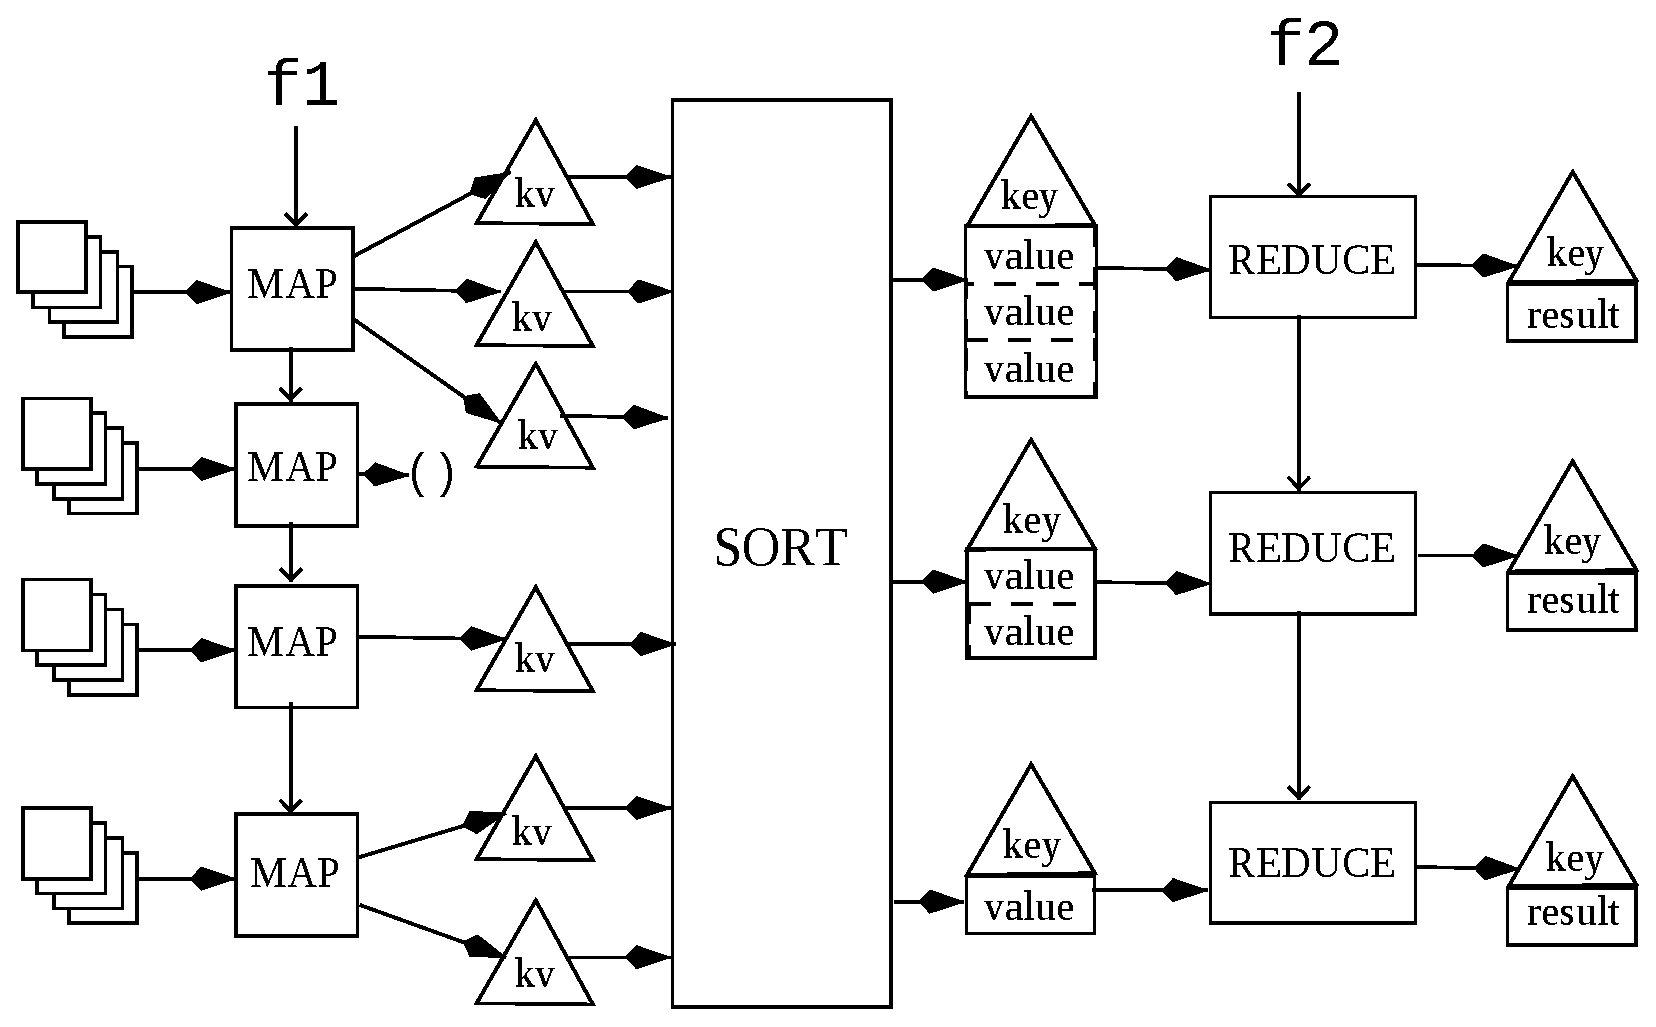
\includegraphics[width=350px]{lecture9/mapreduce.eps}
        \caption{Система MapReduce}
    \end{center}
\end{figure}
Входные данные поступают в систему в виде пар ключ-значение $(k_1, v_1)$.
Функция $f1$ ($mapper$) превращает кажду пару в \emph{список} пар-промежуточных
результатов $(k_2, v_2)$. Функция $sort$ сортирует промежуточные пары по
ключам $k_2$. На вход функции $f2$ ($reducer$) подаются пары вида 
$(k_2, list(v2))$, где второй элемент -- это \emph{список} значений,
соотвестствующих ключу $k_2$. Её результат -- список выходных значений $v_3$.
Таким образом, задача программиста -- это разработать две функции:
\begin{lstlisting}
  mapper (k1, v2) -> list((k2, v2))
  reducer (k2, list(v2)) -> list(v3)
\end{lstlisting}

Технология $MapReduce$ является проприетарной разработкой компании $Google$.
Однако существует открытая реализация этой идеи в системе $Hadoop$. Именно
кластеры $Hadoop$ используются для обработки данных в таких компаниях, как
$Yahoo!$, $Facebook$, $IBM$ и другие.

Мы показали, что как минимум две задачи имеют структуру, подходяющую для
систему $MapReduce$. Это задача умножения матрицы на вектор и задача
подсчёта частоты слов. Можно ли использовать $MapReduce$ для произвольной
задачи?

\section{Списочные гомоморфизмы}
Рассмотрим несколько функций:
\begin{itemize}
\item $map$
\item $length$
\item $sum$
\item $min$
\item $all$
\end{itemize}
Аргументом каждой из функций является список значений. Можно заметить, что
если разбить список-аргумент на несколько частей, то каждую из этих функций
можно вычислить от подсписка, а затем объединить вычисленные значения. Другими
словами, эти функции можно представить в виде
\begin{equation}
  h(x \doubleplus y) = h~x \odot h~y
  \label{eq:1}
\end{equation}
где $\doubleplus$ -- операция конкатенации списков, а $\odot$ -- некоторый
бинарный оператор. Очевидно, что $\odot$ должен быть ассоциативным, т.к.
ассоциативна конкатенация $\doubleplus$. Пример:
\begin{equation*}
  sum(x \doubleplus y) = sum~x + sum~y
\end{equation*}
\begin{equation*}
  length(x \doubleplus y) = length~x + length~y
\end{equation*}

С другой стороны, функцию вычисления наибольшего отсортированного префикса
$lsp$ нельзя представить в таком виде, т.к. $lsp~x$ и $lsp~y$ недостаточно
для вычисления $lsp(x \doubleplus y)$. Эта функция является 
\emph{левосторонней}, т.к. может быть вычислена только \emph{справа} 
\emph{налево}. Аналогично, \emph{правосторонней} функцией будем называть ту,
которая вычисляется \emph{слева} \emph{направо}. Покажем, что если функция
является одновременно и левосторонней и правосторонней, то она удовлетворяет
условию \ref{eq:1}. Такие функции называются \emph{гомоморфизмами}, а 
описанное условие -- третьей теоремой о гомоморфизмах.

\section{Теоремы о гомоморфизмах}
Определение: списочным гомоморфизмом называется функция $h$ такая, что
\begin{equation*}
  h(x \doubleplus y) = h~x \odot h~y
\end{equation*}
где $\odot$ -- ассоциативная операция, а $h~[]$ -- единица для 
$\odot$, т.к. $[]$ является единицей для $\doubleplus$. Т.е.
\begin{equation*}
  h = hom~(\odot)~f~e
\end{equation*}
где $e$ -- начальное значение (единица), $[\cdot]~a = [a]$ и
$h \circ [\cdot] = f$.

Например, можно определить:
\begin{equation*}
  sum = hom~(+)~id~0
\end{equation*}
\begin{equation*}
  length = hom~(+)~one~0 \text{, где } one~a = 1
\end{equation*}

\emph{Левосторонняя} функция $h$ относительно бинарной операции $\oplus$ 
определяется так:
\begin{equation*}
  h([a] \doubleplus y) = a \oplus h~y
\end{equation*}
Проще говоря, функцию $h$ можно записать в виде правой свёртки:
\begin{equation*}
  h = foldr~(\oplus)~e \text{, где } h[] = e
\end{equation*}
Например, для $lsp$:
\begin{equation*}
  a \oplus [] = [a]
\end{equation*}
\begin{equation*}
  a \oplus (b:x) = a:b:x \text{, если } a \leqslant b
\end{equation*}
\begin{equation*}
  a \oplus (b:x) = [a] \text{, иначе }
\end{equation*}
Тогда
\begin{equation*}
  lsp = foldr~(\oplus)~[]
\end{equation*}
Симметрично, \emph{правосторонняя} функция $h$ определяется как 
\begin{equation*}
  h(x \doubleplus [a]) = h~x \otimes a
\end{equation*}
\begin{equation*}
  h = foldl~(\otimes)~e
\end{equation*}
Важно заметить, что операции $\oplus$ и $\otimes$ не обязаны быть 
ассоциативными. Кроме того, можно показать, что
\begin{equation*}
  hom~(\odot)~id~e \text{ -- это \emph{редукция}}
\end{equation*}
\begin{equation*}
  hom~(\doubleplus)~([\cdot] \circ f)~[] \text{ -- это \emph{проекция} map~f}
\end{equation*}

\textbf{Теорема 1.} Каждый гомоморфизм $h$ может быть представлен в виде
композиции редукции и проекции:
\begin{equation*}
  hom~(\odot)~f~e = hom~(\odot)~id~e \circ map~f
\end{equation*}

\textbf{Теорема 2.} Каждый гомоморфизм является правосторонней и левосторонней
функцией:
\begin{equation*}
  hom~(\odot)~f~e = foldr~(\oplus)~e \text{, где } a \oplus s = f~a \odot s
\end{equation*}
\begin{equation*}
  hom~(\odot)~f~e = foldl~(\oplus)~e \text{, где } r \otimes a = r \odot f~a
\end{equation*}

\textbf{Теорема 3.} Если функция $h$ -- одновременно \emph{левосторонняя} и
\emph{правосторонняя}, то $h$ -- гомоморфизм.

Схема доказательства:
\begin{enumerate}
\item Лемма 1: Для любой функции $h$ существует, возможно, частично вычислимая 
  функция $g$ такая, что $h \circ g \circ h = h$.
\item Лемма 2: Если из $h~v = h~x \wedge h~w = h~y$ следует 
  $h~(v \doubleplus w) = h~(x \doubleplus y)$ для любых списков $v, w, x, y$,
  то $h$ -- гомоморфизм. Доказывается через определение оператора $\odot$:
  $t \odot u = h(g~t \doubleplus g~u)$
\item Доказательство теоремы: рассматриваем $h$ поочерёдно как левостороннюю
  и правостороннюю функцию. Показываем, что она удовлетворяет условию второй
  леммы, а, следовательно, является гомоморфизмом.
\end{enumerate}

Практическим примером третьей теоремы является сортировка слиянием (Mergesort)
~\cite{Gibbons95thethird}. 

Понятие списочных гомоморфизмов было введено профессором информатики
и директором компьютерной лаборатории Оксфордского университета
Ричардом Бёрдом~\cite{Bird:1987:ITL:42675.42676}.
\begin{figure}[ht!]
  \begin{center}
    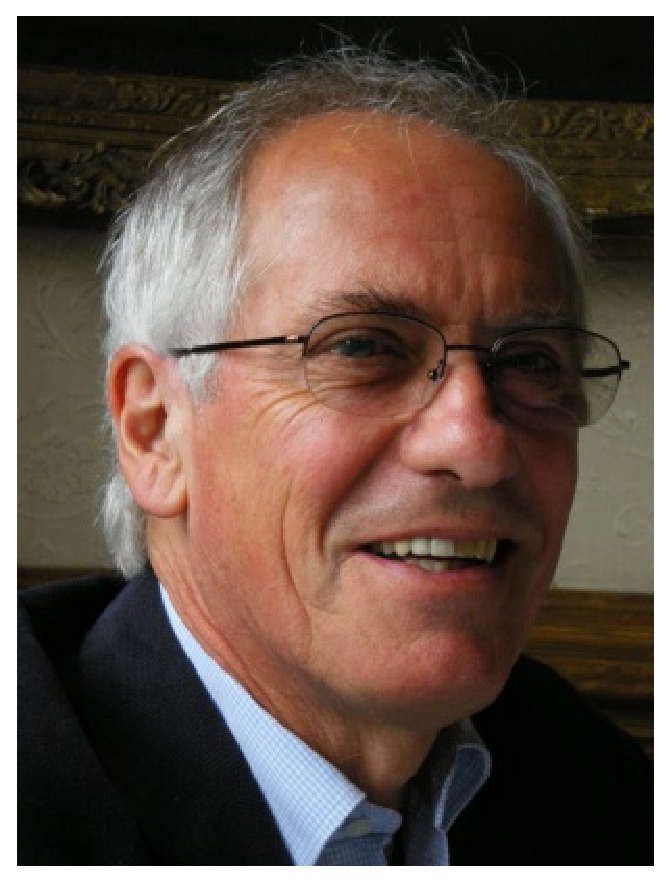
\includegraphics[height=40mm]{lecture9/bird.eps}
    \caption{Ричард Бёрд\\(род. 1943)}
  \end{center}
\end{figure}

Существует ряд исследований, обобщающих понятие списочных гомоморфизмов на
древовидные структуры.
\nocite{*}
\bibliographystyle{alpha}
\bibliography{lecture9}
\end{document}
